\section{Methods and Data: Forecasting Inflation with Machine Learning Models} \label{sec:methods}

The forecasting approach employed in this study adopts an expanding window approach to predict inflation, focusing on a period from January 2015 to January 2024. This methodology allows for the incremental inclusion of new data as it becomes available, thus expanding the training dataset over time and improving the model's adaptability to new economic conditions. The target variable for this analysis is the Consumer Price Index for All Urban Consumers (CPIAUCSL), a common measure of inflation. The CPI data undergoes various transformations to stabilise its variance and improve the predictive performance of the models (set out in \S \ref{sec:methods_data}). These transformations address non-stationarity in the time series data. Several forecasting models are utilised:

\begin{itemize}
    \item \textbf{Random Walk (RW):} This model serves as a naive benchmark, assuming that the best prediction for the next period is the value observed in the current period. It is useful for its simplicity and often performs surprisingly well in financial time series prediction, as noted above in \S \ref{sec:lit_review}.
    \item \textbf{Autoregressive (AR):} This model capitalises on the premise that past values have a linear influence on future values up to `n lags'. It is well-suited for time series data where lagged dependencies are pronounced.
    \item \textbf{Random Forest (RF):} A non-linear model that handles complex interactions between features. It is particularly good at capturing non-linear effects that linear models like AR might miss.
    \item \textbf{Lasso Regression:} Ideal for datasets with many predictors, Lasso helps in feature selection by shrinking the coefficients of less important variables to zero. This is especially valuable in econometric modeling where the researcher is interested in identifying a parsimonious model.
\end{itemize}


The combination of these models provides a robust framework for understanding and forecasting inflation. In addition to the transformed FRED-MD variables, the models employ principal component analysis (PCA) to reduce dimensionality and focus on the most informative aspects of the data, to further enhance the model's effectiveness. Economic datasets often contain a large number of interrelated variables, which can lead to model complexity and computational inefficiency. PCA helps to reduce the dimensionality of the dataset by transforming the original variables into a smaller number of principal components. This makes the dataset more manageable while preserving as much of the critical information as possible. In economic data, predictors can be highly correlated, which complicates the estimation process and can make the model unstable and difficult to interpret. PCA mitigates this by creating principal components that are orthogonal, thus eliminating multicollinearity among them. This stabilisation of the data structure allows for more reliable predictions and interpretations from the models used in the analysis.

The performance of all models is assessed by comparing its forecast accuracy against actual observed values, using error statistics, root mean squared error (RMSE), mean absolute error (MAE), and median absolute deviation (MAD), which are defined as follows:

\begin{equation}
\label{eq:errors}
\begin{aligned}
\operatorname{RMSE}_{m, h} &= \sqrt{\frac{1}{T-T_0+1} \sum_{t=T_0}^T \widehat{e}_{t, m, h}^2}, \\
\operatorname{MAE}_{m, h} &= \frac{1}{T-T_0+1} \sum_{t=T_0}^T\left|\widehat{e}_{t, m, h}\right|, \\
\mathrm{MAD}_{m, h} &= \text{median }\left[\left|\widehat{e}_{t, m, h}-\operatorname{median}\left(\widehat{e}_{t, m, h}\right)\right|\right],
\end{aligned}
\end{equation}


where $\widehat{e}_{t, m, h}=\pi_t-\widehat{\pi}_{t, m, h}$ and $\widehat{\pi}_{t, m, h}$ is the inflation forecast for month $t$, produced by a model $m$ with data up to $t-h$. The first two measures are typical of the forecasting literature. MAD is less common but is useful in capturing the dispersion of predictions, as well as absolute error.



\subsection{Models} \label{sec:methods_models}

\subsubsection{Random Walk Model}

The first benchmark model used is the RW model, which assumes that the best predictor of tomorrow's value is today's value. Formally, the RW model for one-step-ahead forecasts is defined as:
\begin{equation}
    \widehat{y}_{t+h \mid t} = y_t
\end{equation}
for $h=1, \ldots, 12$, where $y_t$ is the last observed value at time $t$. For accumulated forecasts over $h$ months, the forecast is set as:
\begin{equation}
    \widehat{y}_{t+1:t+h \mid t} = y_{t-(h-1):t}
\end{equation}
where $y_{t-(h-1):t}$ represents the accumulated values of the target variable over the previous $h$ months. This model provides a baseline for assessing the predictive power of more complex models.

\subsubsection{Autoregressive Model}

The AR model is a key benchmark in time series forecasting. It utilises historical values of the target variable to predict future values, assuming dependencies only on its own past values. Formally, the AR model is specified as:

\begin{equation}
    y_t = \beta_0 + \sum_{i=1}^{p} \beta_i y_{t-i} + \epsilon_t
\end{equation}

where:
\begin{itemize}[itemsep=0pt,parsep=0pt,topsep=0pt,partopsep=0pt]
    \item $y_t$ represents the value of the target variable at time $t$,
    \item $p$ denotes the number of lags used, indicating the dependency of the forecast on $p$ past observations,
    \item $\beta_0, \beta_1, \ldots, \beta_p$ are coefficients estimated from the data, and
    \item $\epsilon_t$ is the error term, typically assumed to be independently and identically distributed with a mean of zero and constant variance.
\end{itemize}

The parameters are estimated using ordinary least squares (OLS), with the dependent variable being the current value of the target series, and the independent variables are the lagged values of the series. For a model with $n\_lags = p$, the predictor matrix $X$ is constructed as:

\begin{equation}
    X = \begin{bmatrix}
    y_{1} & y_{2} & \cdots & y_{p} \\
    y_{2} & y_{3} & \cdots & y_{p+1} \\
    \vdots & \vdots & \ddots & \vdots \\
    y_{T-p} & y_{T-p+1} & \cdots & y_{T-1}
    \end{bmatrix},
\end{equation}

where $T$ is the total number of observations in the training dataset. Forecasts are generated by applying the estimated model to the lagged values present in the test dataset. This produces a series of one-step-ahead forecasts, facilitating direct comparison between forecasted and actual values.


\subsubsection{Random Forest Model}

In the field of inflation forecasting, RFs offer a robust method that effectively captures the complex, nonlinear interactions among macroeconomic indicators. Conceptually, an RF model consists of numerous decision trees, each partitioning the feature space into segments that yield constant predictions within each segment—typically, the mean of the target values for regression tasks. The model starts with a root node containing the entire dataset and iteratively divides it into smaller nodes by optimising a loss function, usually the mean squared error, which minimises the variance within each node \autocite{Breiman2001RandomForests}.

However, individual decision trees, while detailed, are prone to overfitting—fitting noise rather than signal—and can vary drastically with slight changes in input data. To counteract this, RFs deploy a combination of bootstrapping (sampling random subsets of the training data) and feature bagging (using random subsets of features), to construct each tree. This strategy reduces overfitting by decorrelating the trees’ predictions, enhancing the model's generalisation capabilities to unseen data.

For macroeconomic forecasting, and specifically for predicting inflation trends, RFs are useful because they assess the importance of various predictors, facilitating the identification of the most influential economic indicators. Additionally, the out-of-bag error estimation provides a reliable internal validation mechanism, allowing performance assessment without a separate validation dataset—a significant advantage in fields where data availability may be restricted. The robustness of RFs to overfitting and their capability to handle extensive feature sets without performance degradation make them particularly suited for modeling the intricate dynamics of economic systems, where traditional linear models might fall short.



\begin{figure}[h] 
\label{fig:tree}
\vspace{5mm}
\centering 
\begin{forest}
  for tree={l sep=1.5em, s sep=1.5em, anchor=center, inner sep=0.3em, fill=blue!50, circle, where level=2{no edge}{}}
  [
  Training Data, node box
  [Sample and feature bagging, node box, alias=bagging, above=3em
  [,red!70,alias=a1[[,alias=a2][]][,red!70,edge label={node[above=0.5ex,red arrow]{}}[[][]][,red!70,edge label={node[above=0.5ex,red arrow]{}}[,red!70,edge label={node[below=0.5ex,red arrow]{}}][,alias=a3]]]]
  [,red!70,alias=b1[,red!70,edge label={node[below=0.5ex,red arrow]{}}[[,alias=b2][]][,red!70,edge label={node[above=0.5ex,red arrow]{}}]][[][[][,alias=b3]]]]
  [~~$\dots$~,scale=1.5,no edge,fill=none,yshift=-2em]
  [,red!70,alias=c1[[,alias=c2][]][,red!70,edge label={node[above=0.5ex,red arrow]{}}[,red!70,edge label={node[above=0.5ex,red arrow]{}}[,alias=c3][,red!70,edge label={node[above=0.5ex,red arrow]{}}]][,alias=c4]]]]
  ]
  \node[tree box, fit=(a1)(a2)(a3)](t1){};
  \node[tree box, fit=(b1)(b2)(b3)](t2){};
  \node[tree box, fit=(c1)(c2)(c3)(c4)](tn){};
  \node[below right=0.5em, inner sep=0pt] at (t1.north west) {Tree 1};
  \node[below right=0.5em, inner sep=0pt] at (t2.north west) {Tree 2};
  \node[below right=0.5em, inner sep=0pt] at (tn.north west) {Tree $n$};
  \path (t1.south west)--(tn.south east) node[midway,below=3em, node box] (mean) {Mean in regression or majority vote in classification};
  \node[below=2em of mean, node box] (pred) {Prediction};
  \draw[black arrow={4mm}{3mm}] (bagging) -- (t1.north);
  \draw[black arrow] (bagging) -- (t2.north);
  \draw[black arrow={4mm}{3mm}] (bagging) -- (tn.north);
  \draw[black arrow={4mm}{4mm}] (t1.south) -- (mean);
  \draw[black arrow] (t2.south) -- (mean);
  \draw[black arrow={4mm}{4mm}] (tn.south) -- (mean);
  \draw[black arrow] (mean) -- (pred);
\end{forest}
\caption[Random forest diagram]{A visual representation of a Random Forest model showing sample and feature bagging, decision trees, and the averaging process.\footnotemark}
\end{figure}

\footnotetext{This diagram is based on conceptual material from ``RFs and Decision Trees from Scratch in Python" by Towards Data Science, available at \url{https://towardsdatascience.com/random-forests-and-decision-trees-from-scratch-in-python-3e4fa5ae4249}. Adaptations and modifications were made to the TikZ code originally found on TeX StackExchange at \url{https://tex.stackexchange.com/questions/503883/illustrating-the-random-forest-algorithm-in-tikz}.}


This paper follows the Random Forest method set out in \textcite{Medeiros2021ForecastingMethods}, which is based on the original ideas proposed in \textcite{Breiman2001RandomForests}. This approach constructs a multitude of regression trees on bootstrapped subsets of the data, each tree making local predictions by recursively partitioning the covariate space. A regression tree approximates an unknown nonlinear function by dividing the covariate space into distinct regions, within which the response variable is predicted with a constant estimated from the data. Using an example that draws from \textcite{Hastie2009TheLearning}, given the explanatory variables $X_1$ and $X_2$, the partition might first split on $X_1=s_1$, and subsequent splits on $X_2=s_2$ and $X_1=s_3$, leading to several distinct regions. Within each region $R_k$, the model predicts the dependent variable $Y$ with a constant value $c_k$, calculated as the average of $Y$ values within that region. Each tree is thus a series of binary decisions leading to terminal nodes, where each node corresponds to a region in the input space. The RF model aggregates several such trees to form a robust predictor. This process is visualised in the tree diagram contained in Figure \ref{fig:tree}. Each tree is built on a different bootstrap sample of the dataset, allowing for variations in the structure and splits of each tree. This process helps in reducing the variance of the model without substantially increasing the bias.

Formally, the model for a given dependent variable $\pi_{t+h}$ and a vector of predictors $\boldsymbol{x}_t$ can be described by:
$$
\widehat{\pi}_{t+h} = \frac{1}{B} \sum_{b=1}^B \left[ \sum_{k=1}^{K_b} \widehat{c}_{k, b} \mathbf{I}_{k, b}\left(\boldsymbol{x}_t ; \widehat{\boldsymbol{\theta}}_{k, b}\right) \right]
$$
where:
\begin{itemize}[itemsep=0pt,parsep=0pt,topsep=0pt,partopsep=0pt]
    \item $B$ is the number of bootstrap samples,
    \item $K_b$ is the number of terminal nodes (regions) in the $b$-th tree,
    \item $\widehat{c}_{k, b}$ is the predicted value for region $k$ in bootstrap sample $b$,
    \item $\mathbf{I}_{k, b}$ is an indicator function that is 1 if $\boldsymbol{x}_t$ falls into region $k$ of the $b$-th tree and 0 otherwise, and
    \item $\widehat{\boldsymbol{\theta}}_{k, b}$ are the parameters defining the splits that lead to the $k$-th region in the $b$-th sample.
\end{itemize}

The dataset is prepared by including lagged values of the target variable and applying PCA to reduce dimensionality, forming a comprehensive set of predictors. The RF model utilises these predictors to generate forecasts for each observation in the test dataset. The final forecast for $\pi_{t+h}$ is the average of the forecasts from all trees in the forest, applied to the original data. 

\subsubsection*{Discussion of the Random Forest Model}

The performance of the RF model depends on the appropriate tuning of its hyperparameters, which are selected to optimise the model's accuracy and computational efficiency while ensuring its robustness to overfitting. These parameters are set based on empirical evidence and theoretical considerations, aimed at achieving optimal predictive performance.

\noindent \textbf{Number of Trees:} The number of trees, specified by the hyperparameter \texttt{n\_estimators}, is set to 500. This choice is designed to provide a high level of accuracy while also ensuring that the model's performance stabilises, as increasing the number of trees beyond this point typically yields diminishing returns in terms of error reduction \autocite{Medeiros2021ForecastingMethods}. A larger number of trees enhances the ensemble's ability to generalise, thereby mitigating variance without unduly increasing bias. Choosing a smaller number of trees could lead to increased model variance and potentially underfitting, while an excessively large number might not only waste computational resources but also not yield proportional gains in performance.

\noindent \textbf{Maximum Features per Split:} The hyperparameter \texttt{max\_features} is set to one-third of the total number of features available. This parameter controls the number of features considered when determining the best split at each node of the trees. By restricting the number of features, this setting helps in maintaining a diversity among the trees, preventing the model from fitting too closely to the training data. It strikes a balance between exploring new attribute combinations and retaining prediction accuracy, which is crucial in handling complex economic data structures. Setting \texttt{max\_features} too high could increase the correlation between the trees, reducing the benefit of bagging by making the ensemble too similar to a single decision tree, whereas setting it too low might not capture sufficient information and could increase bias.

\noindent \textbf{Minimum Samples per Leaf:} Set at a minimum of five, the \texttt{min\_samples\_leaf} parameter ensures that each terminal node (leaf) in the tree structures contains no fewer than five data points. This setting helps in preventing the trees from growing overly complex and sensitive to specific samples in the training data, thus enhancing the model's generalisability and robustness against noise and outliers commonly present in economic time series data. A lower threshold might allow the model to capture more detailed information but at the risk of overfitting, while a higher threshold might simplify the model excessively, potentially ignoring valuable information in smaller subsets of data.

\subsubsection{Lasso Model}

The Least Absolute Shrinkage and Selection Operator (Lasso) was introduced by \textcite{Tibshirani1996RegressionLasso} as a modification of the linear regression that incorporates a penalty on the sum of the absolute values of the model coefficients. The method is particularly useful for cases where the number of predictors exceeds the number of observations or when a data set exhibits multicollinearity. The Lasso approach encourages simple, sparse models (i.e., models with fewer parameters).

Formally, the Lasso solution is defined by the following optimisation problem:
\begin{equation}
    \min_{\beta} \left\{ \frac{1}{2n} \sum_{i=1}^n \left( y_i - \beta_0 - \sum_{j=1}^p \beta_j x_{ij} \right)^2 + \lambda \sum_{j=1}^p |\beta_j| \right\},
\end{equation}

where $y_i$ is the dependent variable, $x_{ij}$ is the $j^{th}$ predictor of the $i^{th}$ observation, $\beta_j$ is the coefficient for the $j^{th}$ predictor, $\beta_0$ is the intercept, $\lambda$ is a non-negative regularisation parameter, and $n$ is the number of observations. The penalty term $\lambda \sum_{j=1}^p |\beta_j|$ imposes a constraint on the coefficients that causes some of them to shrink towards zero. This regularisation can significantly reduce the variance of the estimates, at the expense of introducing some bias, hence trading off variance against bias.

In this implementation, the Lasso model is fitted using the \texttt{LassoCV} class from the \texttt{scikit-learn} library, which performs Lasso regression with built-in cross-validation to find the optimal value of $\lambda$. The parameters used in the model fitting included a 5-fold cross-validation (\texttt{cv=5}) and a maximum number of iterations set to 10,000,000 (\texttt{max\_iter=10000000}) to ensure convergence, given the large size of the data set.

To assess the importance and relevance of different predictors in the model, I also compute statistics on the model coefficients. The number of non-zero coefficients (indicative of the model's sparsity), the number of zero coefficients, and the absolute values of the coefficients (indicative of the strength of each predictor) are recorded and analysed in \S \ref{sec:analysis_lasso}.

While Lasso can significantly reduce the risk of overfitting by introducing bias through its regularisation term, the choice of $\lambda$ and the resulting sparsity of the model can have a profound impact on its interpretability and predictive performance. The application of Lasso in inflation forecasting must be done with careful consideration of these trade-offs, particularly in the context of economic data that may exhibit non-standard patterns or noise. This issue is discussed further in \S \ref{sec:analysis_lasso}.



\subsection{Data: FRED-MD} \label{sec:methods_data}

FRED-MD is a large macroeconomic database designed for the empirical analysis of “big data” \autocite{McCracken2016FRED-MD:Research}. The dataset has become a popular resource for modelling US macro variables, due to the number of variables, the length of the time series, and the regularity of updates.

The dataset is of monthly observations, updated on a monthly basis. Each monthly release is referred to as a vintage. A different CSV file is released for each month. The data is publicly accessible.\footnote{The latest vintage, as of the time of publication, is available at: \url{https://files.stlouisfed.org/files/htdocs/fred-md/monthly/2024-04.csv}. The historical vintages can be accessed directly at \url{https://s3.amazonaws.com/files.research.stlouisfed.org/fred-md/Historical_FRED-MD.zip}
} The sample spans from March, 1959 to the present, providing us with a relatively rich data set of macroeconomic time series with $x = 127$ variables and $t = 780$ observations. These variables are grouped under eight headings of macroeconomic indicators: output and income, labour market, consumption and orders, orders and inventory, money and credit, interest rates and exchange rates, prices, and stock market.

As the focus of this paper in inflation forecasting, the dependent variable of interest throughout the analysis is \texttt{CPIAUCSL}. I use the data from January 2015 to January 2024 as the forecasting window throughout the paper. The time series of \texttt{CPIAUCSL} is shown below in Figure \ref{fig:cpi}.

\begin{figure}[H]
    \centering
    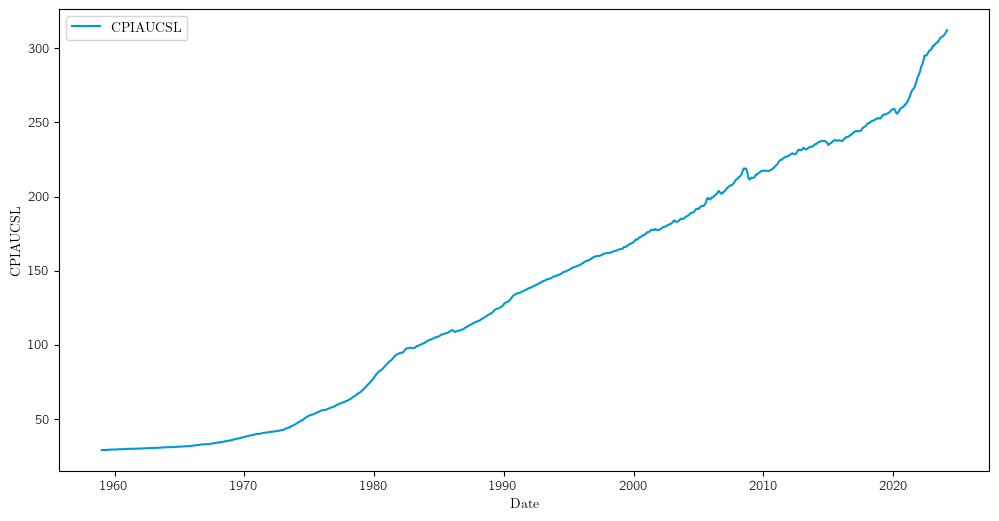
\includegraphics[width=1\linewidth]{figures/cpi.png}
    \vspace{-30pt}
    \caption{CPI, all items, 1960-2024.}
    \label{fig:cpi} 
\end{figure}

A full list of the variables available in FRED-MD is included in the Appendix, in Table \ref{tab:appendix_var}. The data is not stationary by default, but the first row of the data contains the relevant transformations needed to prepare the data. The codes are as follows:

\begin{enumerate}[itemsep=0pt,parsep=0pt,topsep=0pt,partopsep=0pt]
    \item no transformation,
    \item first order difference,
    \item second order difference,
    \item logarithm,
    \item first order logarithmic difference,
    \item second order logarithmic difference, and
    \item percentage change.
\end{enumerate}

In the model, the dataset is divided into two subsets: training data (\texttt{train\_data}) and test data (\texttt{test\_data}). The training data is used to estimate the parameters of the model, while the test data is used to evaluate the model's forecasting ability.


